%!TEX root = ../dokumentation.tex

\chapter{Setup}\label{cha:Setup}
Vor Beginn der Implementierung steht das Setup der Entwicklungsumgebung. Um die Anwendug testen zu können, wird eine \ac{VM} mit dem \ac{OS} Ubuntu verwendet. Auf diesem muss Hadoop installiert und konfiguriert sein. Dabe ist zu beachten, dass es sich um eine Single Node Installation handelt. Es wird also kein Clustering vorgenommen.

Auch in der \ac{IDE} muss ein Setup durchgeführt werden. Dabei handelt es sich, wie auch bei der Konfiguration der \ac{VM}, um Einstellungen, welche nicht im Zusammenhang mit der Umsetzung der Anwendung stehen. Die nachfolgenden Schritte werden so (oder ähnlich) für die Entwicklung aller Hadoop MapReduce Anwendungen vorgenommen.

<Einleitung in das Kapitel noch nicht komplett rund...>

\section{Installation von Hadoop}\label{sec:InstallationHadoop}
Die Installation des Testsystems findet auf einer Linux \ac{VM} mit Ubuntu Version 14.04.2 \ac{LTS} statt, und wird nach der durch Freiknecht beschriebenen Anleitung durchgeführt. 

\subsection{Einrichten eines dedizierten Hadoop-Users}
Dabei wird zunächst ein eigener User, sowie eine eigene Gruppe, für Hadoop angelegt. Dies wird aus Sicherheitsgründen gemacht, da keine Anwendung als Root-User ausgefürt werden darf.

Zusätzlich wird ein \ac{SSH} Zugang für den User angelegt. Hierzu nennt Freiknecht als Gründe zum einen, dass später bei der Verwendung eines Hadoop-Clusters, die Systeme miteinander kommunizeiren müssen, und zum anderen damit, dass auch vom Hostsystem Dateien auf die \ac{VM} abgelegt werden. Für den \ac{SSH}-Zugang muss ein Schlüssel nach dem Verfahren von \ac{RSA} für den User erzeugt und bei den authorisierten Schlüsseln abgelegt. Abschließend, um den Host zu den bekannten Systemen hinzuzufügen, muss der Hadoop User eine erstmalige Verbindung herstellen.\footcite[Vgl.][S. 30 f.]{Freiknecht.2014}

\autoref{lis:KonfHadoopUser} zeigt die Kommandozeilen Befehle für die gerade beschriebenen Aktionen. \\

\begin{lstlisting}[language=bash, caption={Konfiguration des Hadoop Users}, label=lis:KonfHadoopUser]
# Create usergroup and user
sudo addgroup hadoop
sudo adduser -ingroup hadoop hduser

# login as hadoop user and create rsa key
su - hduser
ssh-keygen -t rsa -P ""

# add to authorized keys
cat $HOME/.ssh/id_rsa.pub >> $HOME/.ssh/authorized_keys

# Initial login on host via ssh
ssh localhost
\end{lstlisting}

\subsection{Installation von Hadoop}
Dachdem der dedizierter User angelegt wurde, kann die Installation von Hadoop selbst durchgeführt werden. Hierzu wird zunächst die aktuelle Version von Hadoop in das \textit{/usr/local} Verzeichnis heruntergeladen, entpackt, nach hadoop umbenannt und mit den entsprechenden Berechtigungen für den dedizierten User ausgestattet (\autoref{lis:HerunterladenUndEntpacken}). Im gegensatz zur Anleitung von Freiknecht wird die aktuelle Version 2.7.1 statt 2.2.0 verwendet. \\

\begin{lstlisting}[language=bash, caption={Herunterladen und entpacke von Hadoop}, label=lis:HerunterladenUndEntpacken]
$ cd /usr/local
$ sudo wget http://apache.openmirror.de/hadoop/common/current
            /hadoop-2.7.1.tar.gz
$ sudo tar xfz hadoop-2.7.1.tar.gz
$ sudo mv hadoop-2.7.1 hadoop
$ sudo chown -R hduser:hadoop hadoop
\end{lstlisting}

Da Hadoop in einem extra Verzeichnis installiert wurde, müssen für den User noch eine Reihe von Umgebungsvariablen gesetzt werden. Diese werden der \textit{.bashrc} Datei, welche im Home-Verzeichnis des Users liegt, hinzugefügt. \\

\begin{lstlisting}[language=bash, caption={Umgebungsvariablen für Hadoop}, label=lis:Umgebungsvariablen]
# Java
export JAVA_HOME=/usr/lib/jvm/java-7-openjdk-amd64

# Hadoop
export HADOOP_INSTALL=/usr/local/hadoop
export PATH=$PATH:$HADOOP_INSTALL/bin
export PATH=$PATH:$HADOOP_INSTALL/sbin
export HADOOP_MAPRED_HOME=HADOOP_INSTALL
export HADOOP_COMMON_HOME=HADOOP_INSTALL
export HADOOP_HDFS_HOME=HADOOP_INSTALL
export HADOOP_YARN_HOME=HADOOP_INSTALL
\end{lstlisting}

Abschließend muss die Installation von Hadoop getestet werden, indem der Befehl \textit{hadoop version} in der Komandozeile ausgeführt wird. \autoref{fig:ErgebnisKomandozeileneingabe} zeigt das Ergebnis der Komandozeileneingabe. Die Ausgabe bestätigt die erfolgreiche Installation.\footcite[Vgl.][S. 32 f.]{Freiknecht.2014}

\begin{figure}[h]
	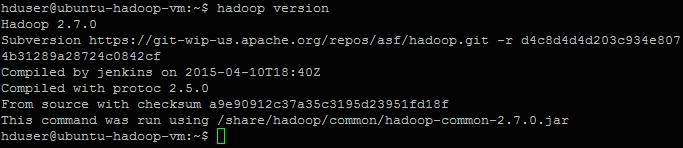
\includegraphics[width=1\textwidth]{hadoop_version.png}
	\caption{Ergebnis für die Komandozeileneingabe \textit{hadoop version}}
	\label{fig:ErgebnisKomandozeileneingabe}
\end{figure}

\subsection{Konfiguration für Pseudo-Distributed Umgebung}
Hadoop kann auch als Single Node installation in einer Pseudo-Distributed Umgebung laufen, in welcher jeder Hadoop Deamon als eigenständiger Java-Prozess ausgefürt wird. Um dies zu ermöglichen sind weitere Konfigurationen notwendig, da für diese Umgebung \ac{HDFS} aktiviert wird.

Die Konfiguration wird nach der Dokumentation von Apache durchgeführt. Dabei werden zunächt in den Dateien \textit{core-site.xml} und \textit{hdfs-site.xml}, welche im Verzeichnis \textit{etc/hadoop} zu finden sind, vorgenommen. \autoref{lis:KonfCoreSite} und \autoref{lis:KonfHDFSSite} zeigen die entsprechenden Konfigurationen. \\

\pagebreak
\begin{lstlisting}[language=XML, caption=Konfiguration in der core-site.xml, label=lis:KonfCoreSite]
<configuration>
	<property>
		<name>fs.defaultFS</name>
		<value>hdfs://localhost:9000</value>
	</property>
</configuration>
\end{lstlisting}

\begin{lstlisting}[language=XML, caption=Konfiguration in der hdfs-site.xml, label=lis:KonfHDFSSite]
<configuration>
	<property>
		<name>dfs.replication</name>
		<value>1</value>
	</property>
</configuration>
\end{lstlisting}

Um die Installation zu testen, muss zunächst eine Formatierung der Knoten vorgenommen werden. Erst nach einer Formatierung ist der Start des Dateisystems möglich. Über den Befehl \textit{jps} können die Anzeige aller laufenden Java-Prozesse möglich. \autoref{lis:TestenDerKonf} zeigt die hierfür notwendigen Befehle. Hadoop bietet zusätzlich ein Web-Interface für die Knoten, welches über \textit{http://localhost:50070/} aufgerufen werden kann. Ein Screenshot des Interfaces ist im Anhang zu finden.\footcite[Vgl.][]{ApacheHadoopDoku.2015} \\

\begin{lstlisting}[caption=Testen der Konfiguration, label=lis:TestenDerKonf]
$ bin/hdfs namenode -format
[...]
$ sbin/start-dfs.sh
[...]
$ jps
1277 DataNode
1337 NameNode
2311 Jps
1533 NodeManager
1566 SecondaryNameNode
$ sbin/stop-dfs.sh
[...]
\end{lstlisting}

%<Beschreibung der Installation. Was muss dabei beachtet werden? Was ist wichtig? Was wird ignoriert?>

\section{Anlegen eines neuen Maven Projektes}


<Noch ein Arbeitstitel. Hier soll es in erster Linie darum gehen wie man ein Projekt für die Entwicklung einer Java Anwendung anlegt, welche Hadoop MapReduce verwenden soll. Maven sollte aus dem Titel raus, da das noch nicht ein mal bis hier hin erwähnt wurde (außer vielleicht kurz in der Definition der Umgebung). Maven muss beschrieben werden, da es nicht ohne weiteres möglich ist eine Hadoop Anwendung zu schreiben ohne Maven.>